%!TEX program = pdflatex
% Full chain: pdflatex -> bibtex -> pdflatex -> pdflatex

\documentclass[lang=cn,11pt]{elegantpaper}
\usepackage{listings}%使用文内代码引用
%代码格式调整
\usepackage{caption}
\usepackage{graphicx, subfig}
\usepackage{subfigure}% 使用子图
\usepackage{url}
\usepackage{enumerate}%序号enumerate
\usepackage{enumitem}
%导言区域要添加以上两个包

\lstset{ %
language=python,                % the language of the code
basicstyle=\footnotesize,           % the size of the fonts that are used for the code
numbers=left,                   % where to put the line-numbers
numberstyle=\tiny\color{gray},  % the style that is used for the line-numbers
stepnumber=2,                   % the step between two line-numbers. If it's 1, each line 
                                % will be numbered
numbersep=5pt,                  % how far the line-numbers are from the code
backgroundcolor=\color{white},      % choose the background color. You must add \usepackage{color}
showspaces=false,               % show spaces adding particular underscores
showstringspaces=false,         % underline spaces within strings
showtabs=false,                 % show tabs within strings adding particular underscores
frame=single,                   % adds a frame around the code
rulecolor=\color{black},        % if not set, the frame-color may be changed on line-breaks within not-black text (e.g. commens (green here))
tabsize=2,                      % sets default tabsize to 2 spaces
captionpos=b,                   % sets the caption-position to bottom
breaklines=true,                % sets automatic line breaking
breakatwhitespace=false,        % sets if automatic breaks should only happen at whitespace
title=\lstname,                 % show the filename of files included with \lstinputlisting;
                                % also try caption instead of title
keywordstyle=\color{blue},          % keyword style
commentstyle=\color{green},       % comment style
stringstyle=\color{red},         % string literal style
escapeinside={\%*}{*)},            % if you want to add LaTeX within your code
morekeywords={*,...}               % if you want to add more keywords to the set
}

\title{TSP 问题及其求解\\ {\small 开题报告}}
\author{\href{https://github.com/LT1st/System_engineering_programm/tree/master}{ 卢韬 }}
\institute{自动化1903班 \\20194127}
%\version{0.07}
%\date{\today}


\begin{document}

\maketitle

\begin{abstract}
\noindent 
\qquad TSP问题已经被研究多年(\cite{tspbookPCB}),已有诸多工作从精确算法(动态规划)、启发式算法(随机贪婪搜索)、亚启发式算法(禁忌搜索(\cite{TSforTSP}))、元启发式算法(遗传算法、粒子群优化(\cite{PSOforTSP}))等方向入手,在获取精确解的能力上取得了较好的效果。然而,由于TSP问题NP难的特点,没有单一的方法能快速、精确地求解各种类型的TSP样例。而这些算法评价指标之间普遍存在着诸多trade-off,单一的求解最优解的能力不足以衡量算法好坏。
因此面对不同特点的算例样本,需要一种科学的评价指标衡量选取哪种算法更好。
本项目将讨论多种用于求解TSP问题算法的原理,并将使用python复现、对比各类算法。最终,结合实验过程和关键评价指标(精度、复杂度、速度)给出一种统一的算法评价指标计算方法,并得到不同特点的算例下最适合的算法。
所有的代码和笔记将开源在:
%引文
\href{https://github.com/LT1st/System_engineering_programm/tree/master}{github开源地址}。\par
\keywords{TSP问题,遗传算法,禁忌搜索,贪婪算法,动态规划算法,粒子群优化算法}
\end{abstract}

\newpage
\tableofcontents
\newpage

\section{TSP问题介绍}
旅行推销员问题(Travelling salesman problem, TSP)描述如下:给定一系列城市和每对城市之间的距离,求解访问每一座城市一次并回到起始城市的最短回路。
它是组合优化中的一个NP难问题,在运筹学和理论计算机科学中非常重要。
TSP问题在 1930 年代在维也纳和哈佛大学首次开始研究,在 1950 年代和 1960 年代在学术界开流行,当时的最优模型可以解决48城市的TSP问题。在1970年代,解决能力达到120维,不久又达到318维。如今,目前的最强模型能求解多达24978维的TSP问题。
从图论的角度来看,该问题实质是在一个带权完全无向图中,找一个权值最小的Hamilton回路\footnote{哈密顿图是一类无向图,从指定的起点前往指定的终点,途中经过所有其他节点且只经过一次。闭合的哈密顿路径称作哈密顿回路。}。由于该问题的可行解是所有顶点的全排列,随着顶点数的增加,会产生组合爆炸。1972 年,Richard Karp 发表了一篇17k引用的论文\cite{nphard},证明了哈密顿循环问题是 NP 完全的。这意味着数学上来说,旅行商问题是 NP 难的。


TSP问题具有实际应用背景。目前被广泛应用于公共服务可靠性、信号控制、路径规划(\cite{tspintranspot})、PCB生产(\cite{tspbookPCB})、流水车间问题及其变体(\cite{bagchi2006review})等诸多实际问题中。

\subsection{TSP问题的数学模型}
对TSP问题有如下数学描述:
\begin{equation}
    \min \sum_{i,j=1}^{n} x_{ij} d_{ij} 
    \label{eq:tsp description}
\end{equation}

Subject to :
\begin{equation}
    \sum_{i\in V} x_{i j}=1 , \forall i \in V_{c}
    \label{eq:binom}
\end{equation}

\begin{equation}
    \sum_{j\in V} x_{i j}=1 , \forall j \in V_{c}
    \label{eq:binom}
\end{equation}

\begin{equation}
    \sum_{i\in S} \sum_{j\in S} x_{i j}\leq \lvert S \rvert - 1  , \forall S \subset V_{c} , 2 \leq \lvert S \rvert \leq n
    \label{eq:binom}
\end{equation}

公式中未知数的含义如表\ref{tab:annotation of the mathematic description}:
\begin{table}[ht]
  \small
  \centering%居中
  \caption{未知数定义 \label{tab:annotation of the mathematic description}}
    \begin{tabular}{c c c c}%表示行数、居中方式
    \toprule
        未知数    &  含义         &        取值范围    &  注释  \\
    \midrule
    $d_{ij}$     &    i到j的距离  &   $[0,-\infty) $  &  距离衡量可以用p范数  \\
    $x_{ij}$     &   在i后访问j   &      0,1         & 使用one-hot编码 \\
    i , j       &   城市代号     &  $i \neq j $       & 不超过城市数量          \\
    N       &   节点集合     &  len(N)=n       &    所有城市的集合       \\
    \bottomrule
    %\multicolumn{4}{l}{\scriptsize Standard errors in parentheses} \\
    %\multicolumn{4}{l}{\scriptsize *** p<0.01, ** p<0.05, * p<0.1} \\
    \end{tabular}%
\end{table}%

\subsection{TSP问题数据集}
TSP问题可用的数据集非常之多,比如\cite{tspdataset}提出的TSPLIB—A、

根据Google公司的一篇文档\footnote{数据详细解释\href{https://docs.google.com/file/d/0B4zUGKjaO9uERU1RZDNuRkg3TW8/edit?resourcekey=0-MRgfJcUZrleab5nfdCOaoQ}{下载地址}}对一般TSP问题测试样例数据的规约,可以得到读取数据集方式,具体读取代码在附录中。

附录中给出了快速下载TSP测试样例\footnote{下载源来源:\href{http://elib.zib.de/pub/mp-testdata/tsp/tsplib/tsp/index.html}{数据集下载地址}}的下载python脚本。

附录中还给出了提取文件夹中所有.tsp样例的python代码。

可以使用\lstinline{G.remove_edges_from(nx.selfloop_edges(G))}来去除自环。
利用图论可视化工具(\cite{NetworkXweb}),可以将邻接矩阵读取并转化为邻接关系数列,并进一步可视化无向图如图\ref{img:TSP数据可视化}。
\begin{figure}[h]
  \centering
  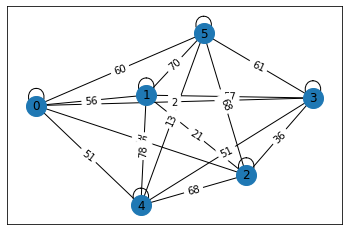
\includegraphics[width=0.5\textwidth]{figure/TSP数据可视化.png} %1.png是图片文件的相对路径
  \caption{TSP数据可视化(蓝色边为可行驶路径。)} %caption是图片的标题
  \label{img:TSP数据可视化} %此处的label相当于一个图片的专属标志,目的是方便上下文的引用
\end{figure}


\subsection{ATSP问题转化为TSP问题}

在上述的TSP问题中,算例给出的通常是城市的二维坐标。i,j两点之间的距离$d_{i,j}$通过欧拉距离(2-范数)计算,因此两点间不同向的边距离是相同的。此类图组成的邻接矩阵有对称性,在图论中形成一个无向图,而这种天然的对称性将解的数量减少了一半。但实际生产过程中,部分问题只能转化为非对称旅行商问题(Asymmetric Travelling Salesman Problem, ATSP),其中$d_{i,j}\neq d_{j,i}$。此类图组成的邻接矩阵无对称性,在图论上可转化为有向图。比如在《现代优化计算方法》课程的实验一中,需要解决的问题就是ATSP。

将未知类似问题转换为特殊情况下的已知问题是常用的手段,因此将ATSP转换为TSP问题求解将有助于扩大TSP求解能力。因此根据其特点,有如下两种方式将ATSP问题转换为TSP问题求解。
\subsubsection{改写距离获取函数}
由于TSP问题给出的邻接矩阵具有对称性,因此TSP算法在设计时就会利用对称性去重\footnote{参考对上三角矩阵的优化储存。}。这样就导致以下三个问题:
\begin{itemize}
    \item .atsp和.tsp测试样例保存的格式不同。
    \item TSP算法中对称邻接矩阵保存的数据结构会降重,导致缺失非对称距离储存能力。
    \item TSP算法中对称邻接矩阵距离读取函数不具备非对称读取能力。
\end{itemize}  

因此想要将TSP算法的求解程序应用到ATSP问题上,一种直接的思路是利用python的重写特性,以上三个位置的函数重写即可。对于启发式算法来说,这样的转化是非常完美的。


\subsubsection{构造新的邻接矩阵}
经过文献检索,我找到了一种将非对称TSP问题转换为对称TSP问题的方法(~\cite{VOLGENANT1983})。
通过这种方法,我们可以将非对称TSP问题转化为对称TSP问题,然后使用适合对称问题的算法求解该问题,而不是重新设计算法。

此算法将一个A称TSP问题的距离矩阵$\boldsymbol{C}$转化为对称TSP问题的距离矩阵$\tilde{\boldsymbol{C}}$。
这样,只需要在读取数据是进行相应转换,就可以无须改动其他代码而直接使用已有TSP求解方法。
算法步骤如下:

1. 令$\overline{\boldsymbol{C}}=\boldsymbol{C}$,其中$\overline{c_{ij}} = - M \quad(i \in N)$。其中M为相当大的数,表示无法通行。

2. 取$\boldsymbol{U_{n\times n}}$为n维方阵。即$\all i,j \in N $, 有$u_{ij}=\infty$。

3. 有ATSP问题的转化对称距离矩阵
%https://blog.csdn.net/zll_hust/article/details/114288869
\begin{equation}
\tilde{\boldsymbol{C}}=
    \left(
        \begin{smallmatrix}
        \boldsymbol{U} & \overline{\boldsymbol{C}}^\mathrm{T} \\
        \overline{\boldsymbol{C}} & \boldsymbol{U}
        \end{smallmatrix}
    \right)
\label{eq:binom}
\end{equation}

4. 此时新的城市节点集合为:
\begin{equation}
\tilde{N}=
    \{1,2, \ldots, n, n+1, \ldots, 2 n\}
\label{eq:binom}
\end{equation}


5. 此时需要转化后TSP问题得到的最优解有以下以下形式:
\begin{equation}
N(i_1) \rightarrow N(i_1+n) \rightarrow N(i_2) \rightarrow N(i_2+n) \rightarrow \ldots \rightarrow N(i_n) \rightarrow N(i_n +n) \rightarrow N(i_1) 
\label{eq:binom}
\end{equation}


其对应的转化函数如下,拼接过程使用了numpy库。
\begin{lstlisting}[language=python][citation=atsp2tsp]
# 为了使算法方便观察,没有使用节省内存和更快的写法,
# 但减少中间变量和新建数组,会显著加快程序运行
def ATSP2TSP_np(matrix):
    lu = np.ones_like(matrix)*(10000)
    ru = matrix.T
    rd = np.ones_like(matrix)*(10000)
    # 先竖着拼接
    left = np.concatenate((lu,matrix),axis=0)
    right = np.concatenate((ru,rd),axis=0)
    # 整体拼接
    return np.concatenate((left, right),axis=1)
\end{lstlisting}





\section{求解TSP问题的算法}
根据所学内容,TSP问题有有如图\ref{img:算法汇总}常用算法。总体分为精确算法、启发式算法和深度学习算法。

\begin{figure}[h]
  \centering
  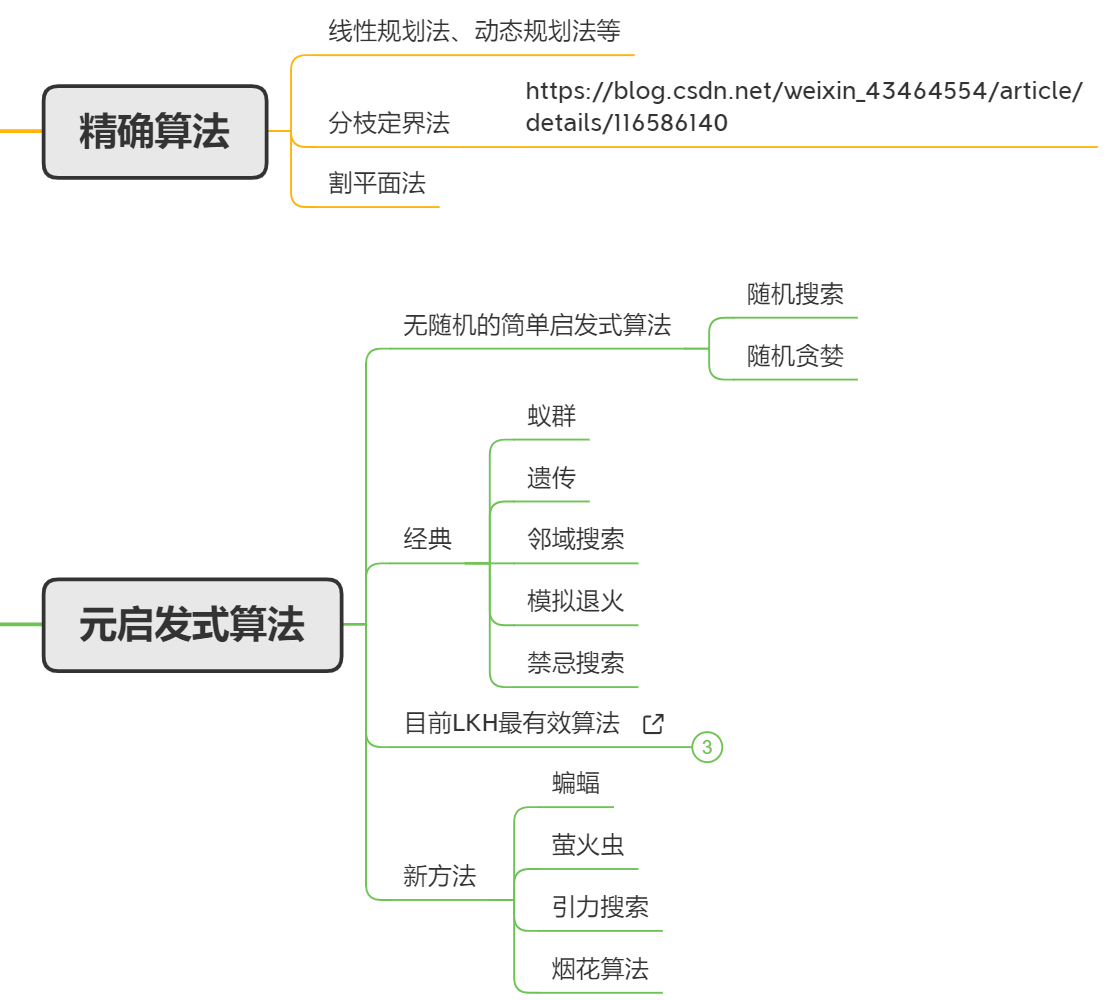
\includegraphics[width=0.8\textwidth]{figure/算法汇总.png} %1.png是图片文件的相对路径
  \caption{算法汇总 } %caption是图片的标题
   %此处的label相当于一个图片的专属标志,目的是方便上下文的引用
   \label{img:算法汇总}
\end{figure}

\subsection{精确算法}
最直接的求解算法是对所有可能的路径进行完整枚举,以确定成本最低的路径。然而,对于n个城市求解的时间复杂度为$O(n!)$时间,这种方法仅适用于较小的城市规模。

\subsubsection{分支定界法}
根据2021秋季学期课程《系统优化与人工智能》和《系统工程概论》,分支定界方法常用于求解各类优化问题。

 ILP 首先被宽松并使用 Simplex 方法作为 LP 求解,然后通过枚举整数变量重新获得可行解。



\subsubsection{线性规划算法}

\subsubsection{动态规划算法}

\subsection{启发式算法}
NP-hard 问题难以在大尺度上以最优方式精确求最优解。启发式算法常用于给出一个好的近似解,但不一定是最优解。这些算法不保证最优解,但在合理的计算时间内给出接近最优的解。

\subsection{深度学习算法}
基于深度学习的算法准确率已经接近经典方法。但目前效率仍然较差,在数百节点左右的规模上就很难快速收敛。因此无法将学习到的策略推广到实际规模的更大实例。~\cite{goodDLforTSP}的工作将目前主流的深度学习技巧重新整合,并提出了合适的网络结构和学习方式。同时其开源代码已有较多使用量,非常成熟。



\section{禁忌搜索算法}
\subsection{禁忌搜索算法求解TSP问题}
禁忌搜索(Tabular Search,TS)最初由\cite{tabusearch}提出。禁忌搜索是一种亚启发式随机搜索算法,它从一个初始可行解出发,通过随机指定的变化规则(比如2-gram),选择实现让特定的目标函数值变化最多的移动。本质上是通过扩大邻域搜索结构来得到更好的解。为了避免陷入局部最优解,TS搜索中采用了禁忌表作为记忆机制。对已经试探过得较优解,能在一定时间内避免尝试从而避免震荡求解的情况。


\begin{figure}[h]
  \centering
  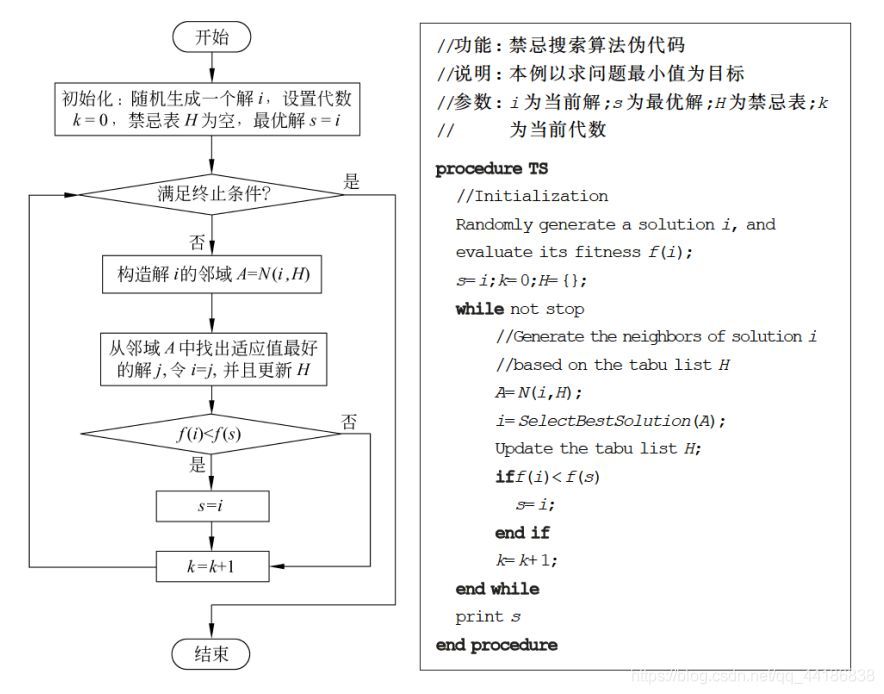
\includegraphics[width=0.8\textwidth]{figure/禁忌搜索算法流程.jpg} %1.png是图片文件的相对路径
  \caption{禁忌搜搜算法求解TSP问题思路 } %caption是图片的标题
   %此处的label相当于一个图片的专属标志,目的是方便上下文的引用
   \label{tabsearch}
\end{figure}

根据算法介绍,可以得到流程框图,如图~\ref{tabsearch}。

\subsubsection{算法关键要素}
1. 禁忌对象的选取(禁忌表中被禁的那些变化元素)

        \begin{itemize}[leftmargin=50pt]
        \item 解的简单变化:将原来的解和变化后的解都记录下来。如:$ABCDE \rightarrow ACBDE  $
        \item 向量的变化:记录变化位置和变化量。如:
            $(1,1,0,1,0,1) \rightarrow (1,0,0,1,0,1)    $
        \item 目标值的变化 : 禁止相同目标值的解被接受。如:
            $f(x)$。
        \end{itemize}

2. 邻域结构(决定邻域按什么样的方式生成)
        \begin{itemize}[leftmargin=50pt]
        \item 使用k-opt,既交换当前解级的k个城市。
            $(123456) \rightarrow (126543)    $
        \item 比如~\cite{2opt}中使用的2-opt方法,每次交换两个城市,如$(123456) \rightarrow (123465)    $。
        \end{itemize}

3. 禁忌长度的确定(被禁对象不允许选取的迭代代数,tabu(x) = t )
        \begin{itemize}[leftmargin=50pt]
        \item t为给定常数。
        \item t为某一范围。
        \item t动态变化,比如我使用的余弦下降、幂指数下降等策略。
        \end{itemize}
4. 特赦规则(aspiration criteria)
        \begin{itemize}[leftmargin=50pt]
        \item 基于评价值的规则:遇到更好的解。
        \item 基于最小错误的规则:当所有对象都被禁忌时,选择最好。
        \item 基于影响力的规则:对目标函数的影响大小。
        \end{itemize}
5. 候选集合的确定
        \begin{itemize}[leftmargin=50pt]
        \item 选择邻域中目标值最佳的若干个邻居。
        \item 随机选取。
        \end{itemize}
6. 终止规则
        \begin{itemize}[leftmargin=50pt]
        \item 确定步数终止:迭代代数超过给定值K,终止计算。
        \item 频率控制原则:某一解、目标值、元素序列的频率超过给定                                   标准,终止计算。
        \item 目标控制原则:给定步数内目标值没有改进。
        \item 目标值偏离程度原则:$f(x) - Z_{LB} \leq \epsilon$。
        \end{itemize}

\subsubsection{算法实现}
根据如图\ref{img:禁忌搜索算法}算法探究,我完成了使用禁忌搜索的TSP求解。这里我选择了ATSP作为测试样例,但是本质上与TSP都是相通的。此类问题有两个思路,转换为TSP或者按照ATSP的非对称路径来读取。我将两种思路都实现了,最终对比发现后者在储存、速度上都更好。

\subsubsection{算法优化}
本模型首次完成时间较早,但是算法性能始终不好,因此反复尝试了一些技巧来提升性能。从最初的2500+(最好)到现在的1900+(最好)。本次实验的代码完全由本人完成,没有借鉴任何代码。

由于算法从零开始实现,因此数据结构的选取、迭代过程中中间数据的处理等细节有诸多实现方法。因此在完成实验内容后,我利用python中的修饰器技巧,通过函数包装来快速获取各个函数的运行时间,便于找到耗时的瓶颈位置。只需要在写好的函数上加入@timmer即可在调用过程中自动记录时间。此方法来源于我的个人博客,在初学python时候记录的笔记。

%跨页会导致报错
\begin{lstlisting}[language=python][citation=timmer]
import time
def timmer(func):    #传入的参数是一个函数
    def deco(*args, **kwargs): #本应传入运行函数的各种参数
        print('\n函数:{_funcname_}开始运行:'.format(_funcname_=func.__name__))
        start_time = time.time()#调用代运行的函数,并将各种原本的参数传入
        res = func(*args, **kwargs)
        end_time = time.time()
        print('函数:{_funcname_}运行了 {_time_}秒'
              .format(_funcname_=func.__name__, _time_=(end_time - start_time)))
        return res#返回值为函数
    return deco
\end{lstlisting}

最终在算法运行速度优化上有总体85\%时间优化。比如在读取距离方法、ATSP问题处理等多个算法耗时的瓶颈处做了消融实验,选取了运行速度更快的解决方案。同时在算法书写时也使用lamda表达式排序等方法尽量减少代码复杂度。在执行时间判断函数过程中,使用了jupyter notebook独有的魔术指令\lstinline{\%\%!},在每个单元格中都运行多次同一份代码,求取平均值作为最终结果。下图记录的是数据结构的决定。

\subsubsection{训练过程参数控制}
为了保证算法的泛化性能,在代码实现过程中将所有可控变量解耦合。用较多的封装保证算法可以很容易的进行参数调节。在run()函数中,可以通过改变超参数传入,容易的完成各项功能的消融实验。下表所示的是算法的超参数单独单元定义。

\begin{lstlisting}[language=python][citation=varient]
# 算法需要的变量
tabLength = 50                   # 禁忌表长
banned_Table = []                # 禁忌表
city_Num = tab_np.shape[0]       # 城市数
cityNum = tab_np.shape[0]
randSeed = 42                    # 随机数种子
random.seed(randSeed)            # 给random库设计随机数生成器
maxIter = 1000                   # 终止准则
neighborNum = 20000              # 生成的邻居数量
solution = list(range(city_Num)) # 解
solution_list = []               # 生成多个解构成的数组
exchange_Num  = 2                # 领域交换量 2-opt
# 当前路径长度(加一个变化的权重,路径长度和value不一样,非线性,比如平方)
# 加大对离谱解的惩罚力度,但要小心震荡
thisLength = 1000000
thisValue = 1000000
random_accept= 0.05              # 随机接受概率
\end{lstlisting}


同时我也结合自己在深度学习中学习的技巧,将lerning rate(tabu长度)下降、抖动(长时间梯度不下降就跳开)、允许随机犯错等手段加入了算法实现过程中,尽可能优化算法。

观察到表长度较小的时候,很容易出现算求解来回震荡的情况。因此算法需要在表长衰减时候做截断,来保证搜索能力。

\section{粒子群优化算法}
\subsection{粒子群算法介绍}


根据PSO课程上记录的笔记(图\ref{img:PSO笔记}),可以得到算法的流程图和重要参数。
\begin{figure}[h]
  \centering
  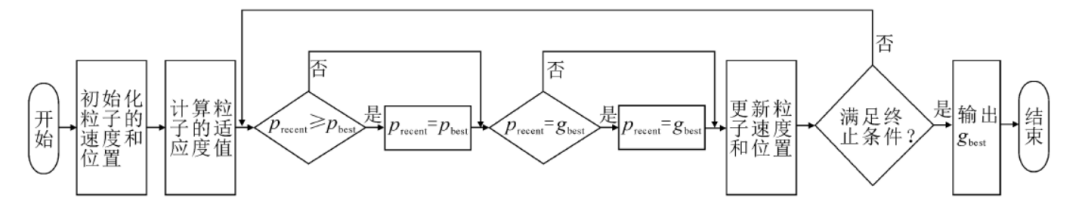
\includegraphics[width=0.7\textwidth]{figure/PSO/粒子群算法标准流程.png} %1.png是图片文件的相对路径
  \caption{粒子群算法标准流程} %caption是图片的标题
  \label{img:粒子群算法标准流程}
\end{figure}
\subsection{超参数(粒子个数、迭代次数等)对搜索性能的探究}
由于PSO算法性能很大程度上取决于超参数选取,因此想要达到更好的性能,需要对超参数进行详细对照实验。
但是使用整体算法求解TSP问题时速度较慢,很长时间才能得到最后的解,不利于调参。所以这里先选用几个常用的测试函数对算法进行大致探索研究,再将其迁移到现有问题上。

这里选用Griewark函数、Rastrigrin函数和Rosenbrock函数三种典型测试函数。根据实验结果和TSP问题特性来做具体参数选择。

观察PSO算法在粒子个数分别设置为50、 100和300,迭代次数分别设置为100、 500和1000情况下的寻找最优解的过程。
\subsubsection{使用对数坐标系进行可视化}
当使用30维的多变数扩展测试函数时,算法搜索范围可以达到(1e0,1e9),跨度很大。如下图\ref{fig:坐标变换效果对比}(a)所示,可以观察到三种颜色表示的三种参数下的三条曲线紧贴在一起,无法直观观察的算法的搜索过程。

\begin{figure}[ht]
\centering    %居中
    \subfigure[] %第一张子图
    {
    	\begin{minipage}{7cm}
    	\centering          %子图居中
    	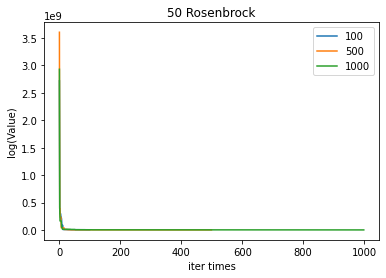
\includegraphics[scale=0.4]{figure/PSO/使用正常坐标系的三种下降曲线.png}   %以pic.jpg的0.5倍大小输出
    	\end{minipage}
    }
    \subfigure[] %第二张子图
    {
    	\begin{minipage}{7cm}
    	\centering      %子图居中
    	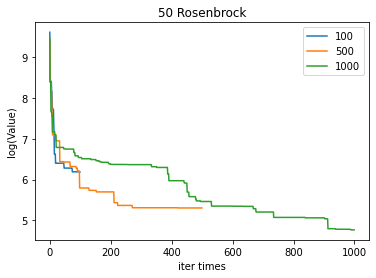
\includegraphics[scale=0.4]{figure/PSO/对数坐标系下的三种下降曲线.png}   %以pic.jpg的0.5倍大小输出
    	\end{minipage}
    }
\caption{坐标变换效果对比} %  %大图名称
\label{fig:坐标变换效果对比}  %图片引用标记
\end{figure}

因此,考虑到模电和自控原理中bode图的对数坐标系,我将数据进行了对数化,使用纵轴为对数坐标系的方法,使得不同参数情况下算法的可视化可以直观体现出来(如图\ref{fig:坐标变换效果对比}(b))。具体实现时,可以采用matplotlib的对数系,也可以采用numpy将数据整体转换,还可以手工转换。这里为了更好体现算法细节,使用手写转换方式。

观察到三条曲线成功分离开了,便于算法性能的对比研究。
但是也要注意,对尺度进行缩放也导致差距较为接近的两条线水平方向重合,其斜率也被去了对数,变化趋势不敏感。因此对于算法执行末期,数量级差距不大情况下,还应该回到标准坐标系下探究。


\subsection{算法实现}
同时,吸取前两次实验中算法实现使用顺序结构的弊端。设置过多全局变量定义的超参数导致进行重复实验时出现变量泄露等问题,这些问题在python中(尤其是jupyter notebook中)debug很困难。此次算法实现用类来封装,超参数使用类内变量,使得创建和销毁都更安全,做多组对照实验时出现问题较少。

同时,由于整体算法在求解TSP问题时速度较慢,不利于调参。这里先选用几个常用的测试函数对算法进行大致探索研究,再将其迁移到现有问题上。

这里选用Griewark函数、Rastrigrin函数和Rosenbrock函数三种典型测试函数。

\subsection{对照试验}
\subsubsection{实验设计}
考虑到实验中涉及到三组变量:目标函数、迭代次数、种群量。为了直观展现这些变量之间的关系,我使用了matplotlib的子图绘制和隐函数的迭代器,可以方便的进行重复对照实验。
同时,我也使用了变量控制,每个子图中的三条下降曲线都只有一个超参数变化。比如:当使用50种群搜索rosenbrock函数时,迭代次数分别设置为100、500、1000进行试验,其图像放置于大图\ref{img:对迭代次数的探究}的(1,1)位置。

图中:
表头为次小图中实验的两个固定参数,用于固定此2参数,比对图例中的参数。大图中的9个小图表示不同参数情况下的运行情况,用于比对其余两参数的情况。

\subsubsection{实验分析}
从图\ref{img:对迭代次数的探究}可以看到不论对于何种函数或采用何种规模种群,其中总存在非常大的“平台期”\footnote{既多个迭代次数后算法达到的最优解没有更新。},也存在有平台期对应的拐点。比如观察到对于Rastrigrin和Griewark函数,在250iter后搜索的边际效益逐渐降低,种群已经逐步落入局部最优的陷阱,很难再有进步。继续增加iter,算法几乎没有进步。而对于Rosenbrock函数,由于其搜索难度较大,因此更多的迭代次数能显著增加结果的最优性。根据100次的重复实验,也可以判断对Rosenbrock函数,其搜索结果与迭代次数具有较强线性相关性。

\begin{figure}[h]
  \centering
  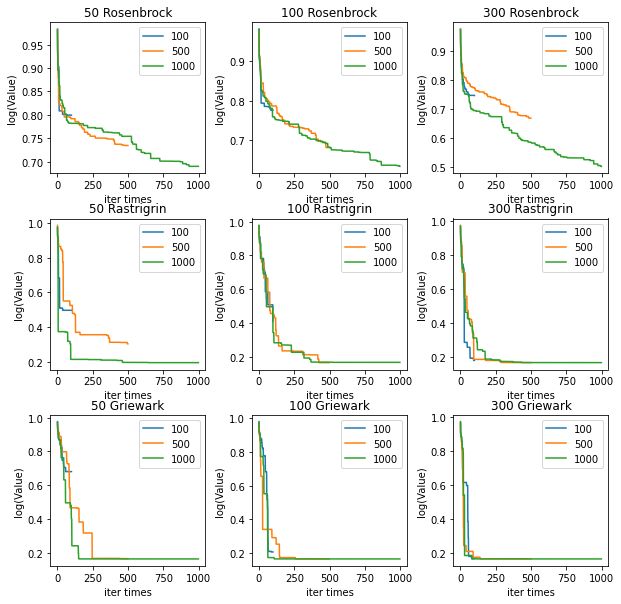
\includegraphics[width=0.5\textwidth]{figure/PSO/对迭代次数的探究.png} %1.png是图片文件的相对路径
  \caption{对迭代次数的探究} %caption是图片的标题
  \label{img:对迭代次数的探究}
\end{figure}

通过衰减速率来看(需要注意的是,图示衰减速率取了对数,但不影响大小关系),大的种群能有更持久的搜索能力,图\ref{img:对种群大小的探究}(2,1)、图\ref{img:对种群大小的探究}(2,3)可以明显看出较小的种群容易陷入某个局部最优值,而种群数量大就有更多机会持续找到更优的局部最优值。既对于大多数情况,大种群的收敛位置要由于小种群。这样的想法也在更大规模、更细密的采样上得到了实验。这里推荐使用google的colab pro平台,其提供的服务器使用多个Intel(R) Xeon(R) CPU @ 2.20GHz,运行速度要比本地快很多,支持了本次大规模测试。我也共享了我的代码,连接在最前方。
\begin{figure}[h]
  \centering
  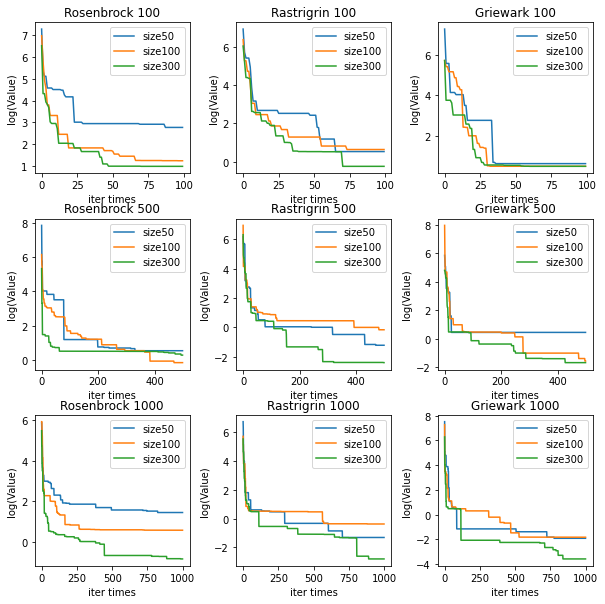
\includegraphics[width=0.5\textwidth]{figure/PSO/对种群大小的探究.png} %1.png是图片文件的相对路径
  \caption{对种群大小的探究} %caption是图片的标题
  \label{img:对种群大小的探究}
\end{figure}


但是同时,我通过做额外的对照试验(图\ref{img:种群量额外的对照实验})发现,过大的种群(5000)反而会导致收敛非常慢,计算时间也呈指数倍增长。而且根据问题不同,搜索算法也不是一定会明显更好。种群规模与算法效率、算法性能之间存在trade-off,需要在具体实现测试样例中分析合适的参数取值。比如在griewark测试样例中,算法性能就没有明显提升。

\begin{figure}[ht]
  \centering
  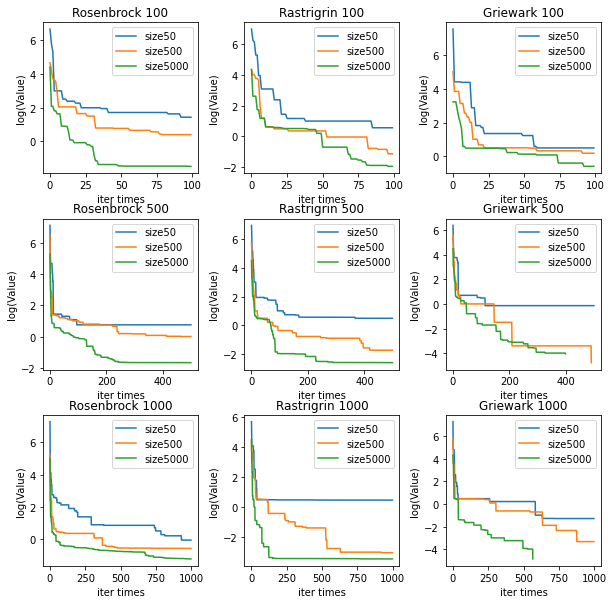
\includegraphics[width=0.5\textwidth]{figure/PSO/种群量额外的对照实验(种群量为50、500、5000).png} %1.png是图片文件的相对路径
  \caption{种群量额外的对照实验(种群量为50、500、5000)} %caption是图片的标题
  \label{img:种群量额外的对照实验}
\end{figure}

这里运算计算时间利用python的修饰器完成,既将计算函数传入@开头的另一个修饰器函数中。

也可以使用tqdm的迭代器来完成(如图\ref{img:不同种群量计算耗时分析}),还可以用python自带的分析测试工具完成。观察到计算时间随着种群数量指数级上升,图中也展示了多次运行求平均(减少随机性干扰)的思想。需要注意的是,python中可以使用魔术指令\%timeit(或者cProfile分析)来自动重复运行单元格,获取平均算法耗时,但是多次运行后,部分变量会被系统优化进入L2chahe缓存、或者被其他解释器自带优化方法优化,其统计的平均耗时将会小于真实情况。因此手写重复运算可能是更合适的方法,这样内循环的变量会被python自动回收,不会被机器优化。

\begin{figure}[ht]
  \centering
  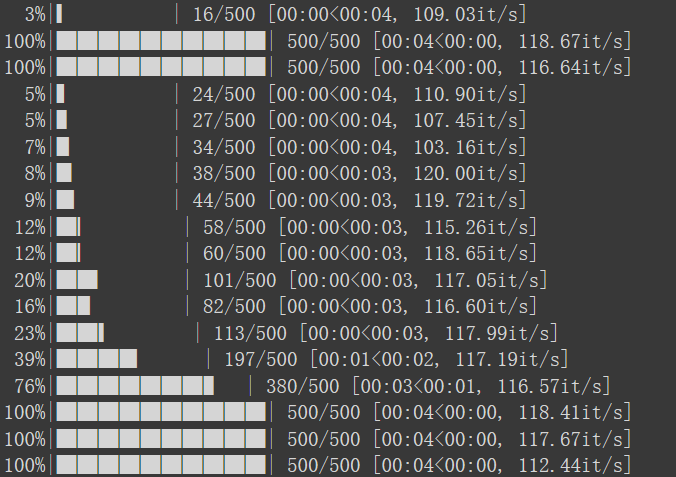
\includegraphics[width=0.4\textwidth]{figure/PSO/提前停止位置(W从0.05增加到1).png} %1.png是图片文件的相对路径
  \caption{不同种群量计算耗时分析(单位:每秒多少次迭代)} %caption是图片的标题
  \label{img:不同种群量计算耗时分析}
\end{figure}









\section{总体算法实现、代码亮点}
\subsection{可复现性}
随机性
运行环境:线上平台、requirement.txt

\subsection{可视化}
如图\ref{img:同随机数种子},本项目使用了matplotlib 中的可视化方法,并加以封装。同时通过训练过程中数据结构保存中间结果,便于直观感受算法运行情况,给出调参数的方向。
\begin{figure}[ht]
  \centering
  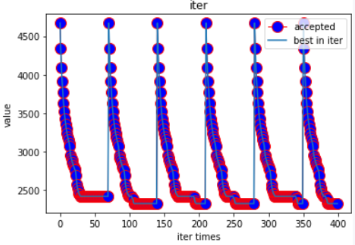
\includegraphics[width=0.4\textwidth]{figure/同随机数种子、同初始解多次运行结果.png} %1.png是图片文件的相对路径
  \caption{同一个初始解进行多次搜索} %caption是图片的标题
  \label{img:同随机数种子} %此处的label相当于一个图片的专属标志,目的是方便上下文的引用
\end{figure}

使用了tqdm库,来可视化算法的训练进程。在大规模测试情况下得以判断运行时间。

\subsection{TSP问题路径可视化}
使用复杂网络处理工具networkx\footnote{\href{https://networkx.org/documentation/stable/auto_examples/index.html}{复杂网络工具networkx}}(\cite{NetworkXpaper})有助于直观展示算法效果。比如环的散乱程度(图\ref{img:TSP路径可视化})。
此方法将\lstinline{numpy.ndarray}格式的临界矩阵数据经过方阵检查、编号、去重复等处理转化为邻接表,进而可视化。


\begin{figure}[ht]
  \centering
  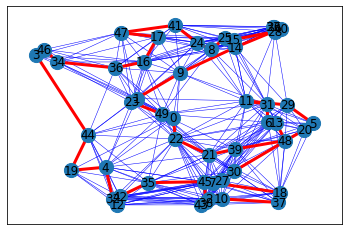
\includegraphics[width=0.4\textwidth]{figure/TSP路径可视化.png} %1.png是图片文件的相对路径
  \caption{TSP路径可视化(其中红色边为最终结果,蓝色边为可行驶路径。)} %caption是图片的标题
  \label{img:TSP路径可视化} %此处的label相当于一个图片的专属标志,目的是方便上下文的引用
\end{figure}

\subsection{调试工具}
\subsubsection{算法效率}


\subsubsection{算法可靠性}
使用warning、assert等错误处理机制,便于切换测试样例带来问题的排查。



%\figref{img:禁忌搜索算法} 引用图







% \nocite{en1,en2}
\clearpage 
% If you want change the bibliography style, replace aer with the prefered one.
\bibliographystyle{aer}

\bibliography{wpref}%导入bib包,这是包的名字

\clearpage 
\appendix
\section{附录}
附录中存放过长的代码和尺寸过大的图片。
\subsection{程序代码}
\begin{lstlisting}[language=python][citation=getdataset]
# 获取数据集
import requests,os
from lxml import etree
from urllib.parse import urlparse
url = 'http://elib.zib.de/pub/mp-testdata/tsp/tsplib/tsp/index.html'
resp = requests.get(url)
text = resp.text
html = etree.HTML(text)
parse = urlparse(url)
root = 'http://elib.zib.de/pub/mp-testdata/tsp/tsplib/tsp/'
for a in html.xpath('//li/a'):
    name = a.xpath('./@href')[0]
    path = os.path.join('res', name)
    if os.path.exists(path):
        print('已存在%s' % name)
        continue
    durl = root + name
    dresp = requests.get(durl)
    with open(path, 'w') as fp:
        fp.write(dresp.text)
    print(name)
\end{lstlisting}

\begin{lstlisting}[language=python][citation=getdataset]
# 读取文件夹下所有.tsp文件
import os
import pandas as pd
path = "./" #文件夹目录
files= os.listdir(path) #得到文件夹下的所有文件名称
s = []
for file in files: #遍历文件夹
     if not os.path.isdir(file) and file[-4:-1]==".tsp" #判断是否是文件夹,不是文件夹才打开
    df = pd.read_csv(file,sep=" ",hearder=None)
    s.appned(df)
print(s) #打印结果
\end{lstlisting}

\subsection{图片}
\begin{figure}[ht]
  \centering
  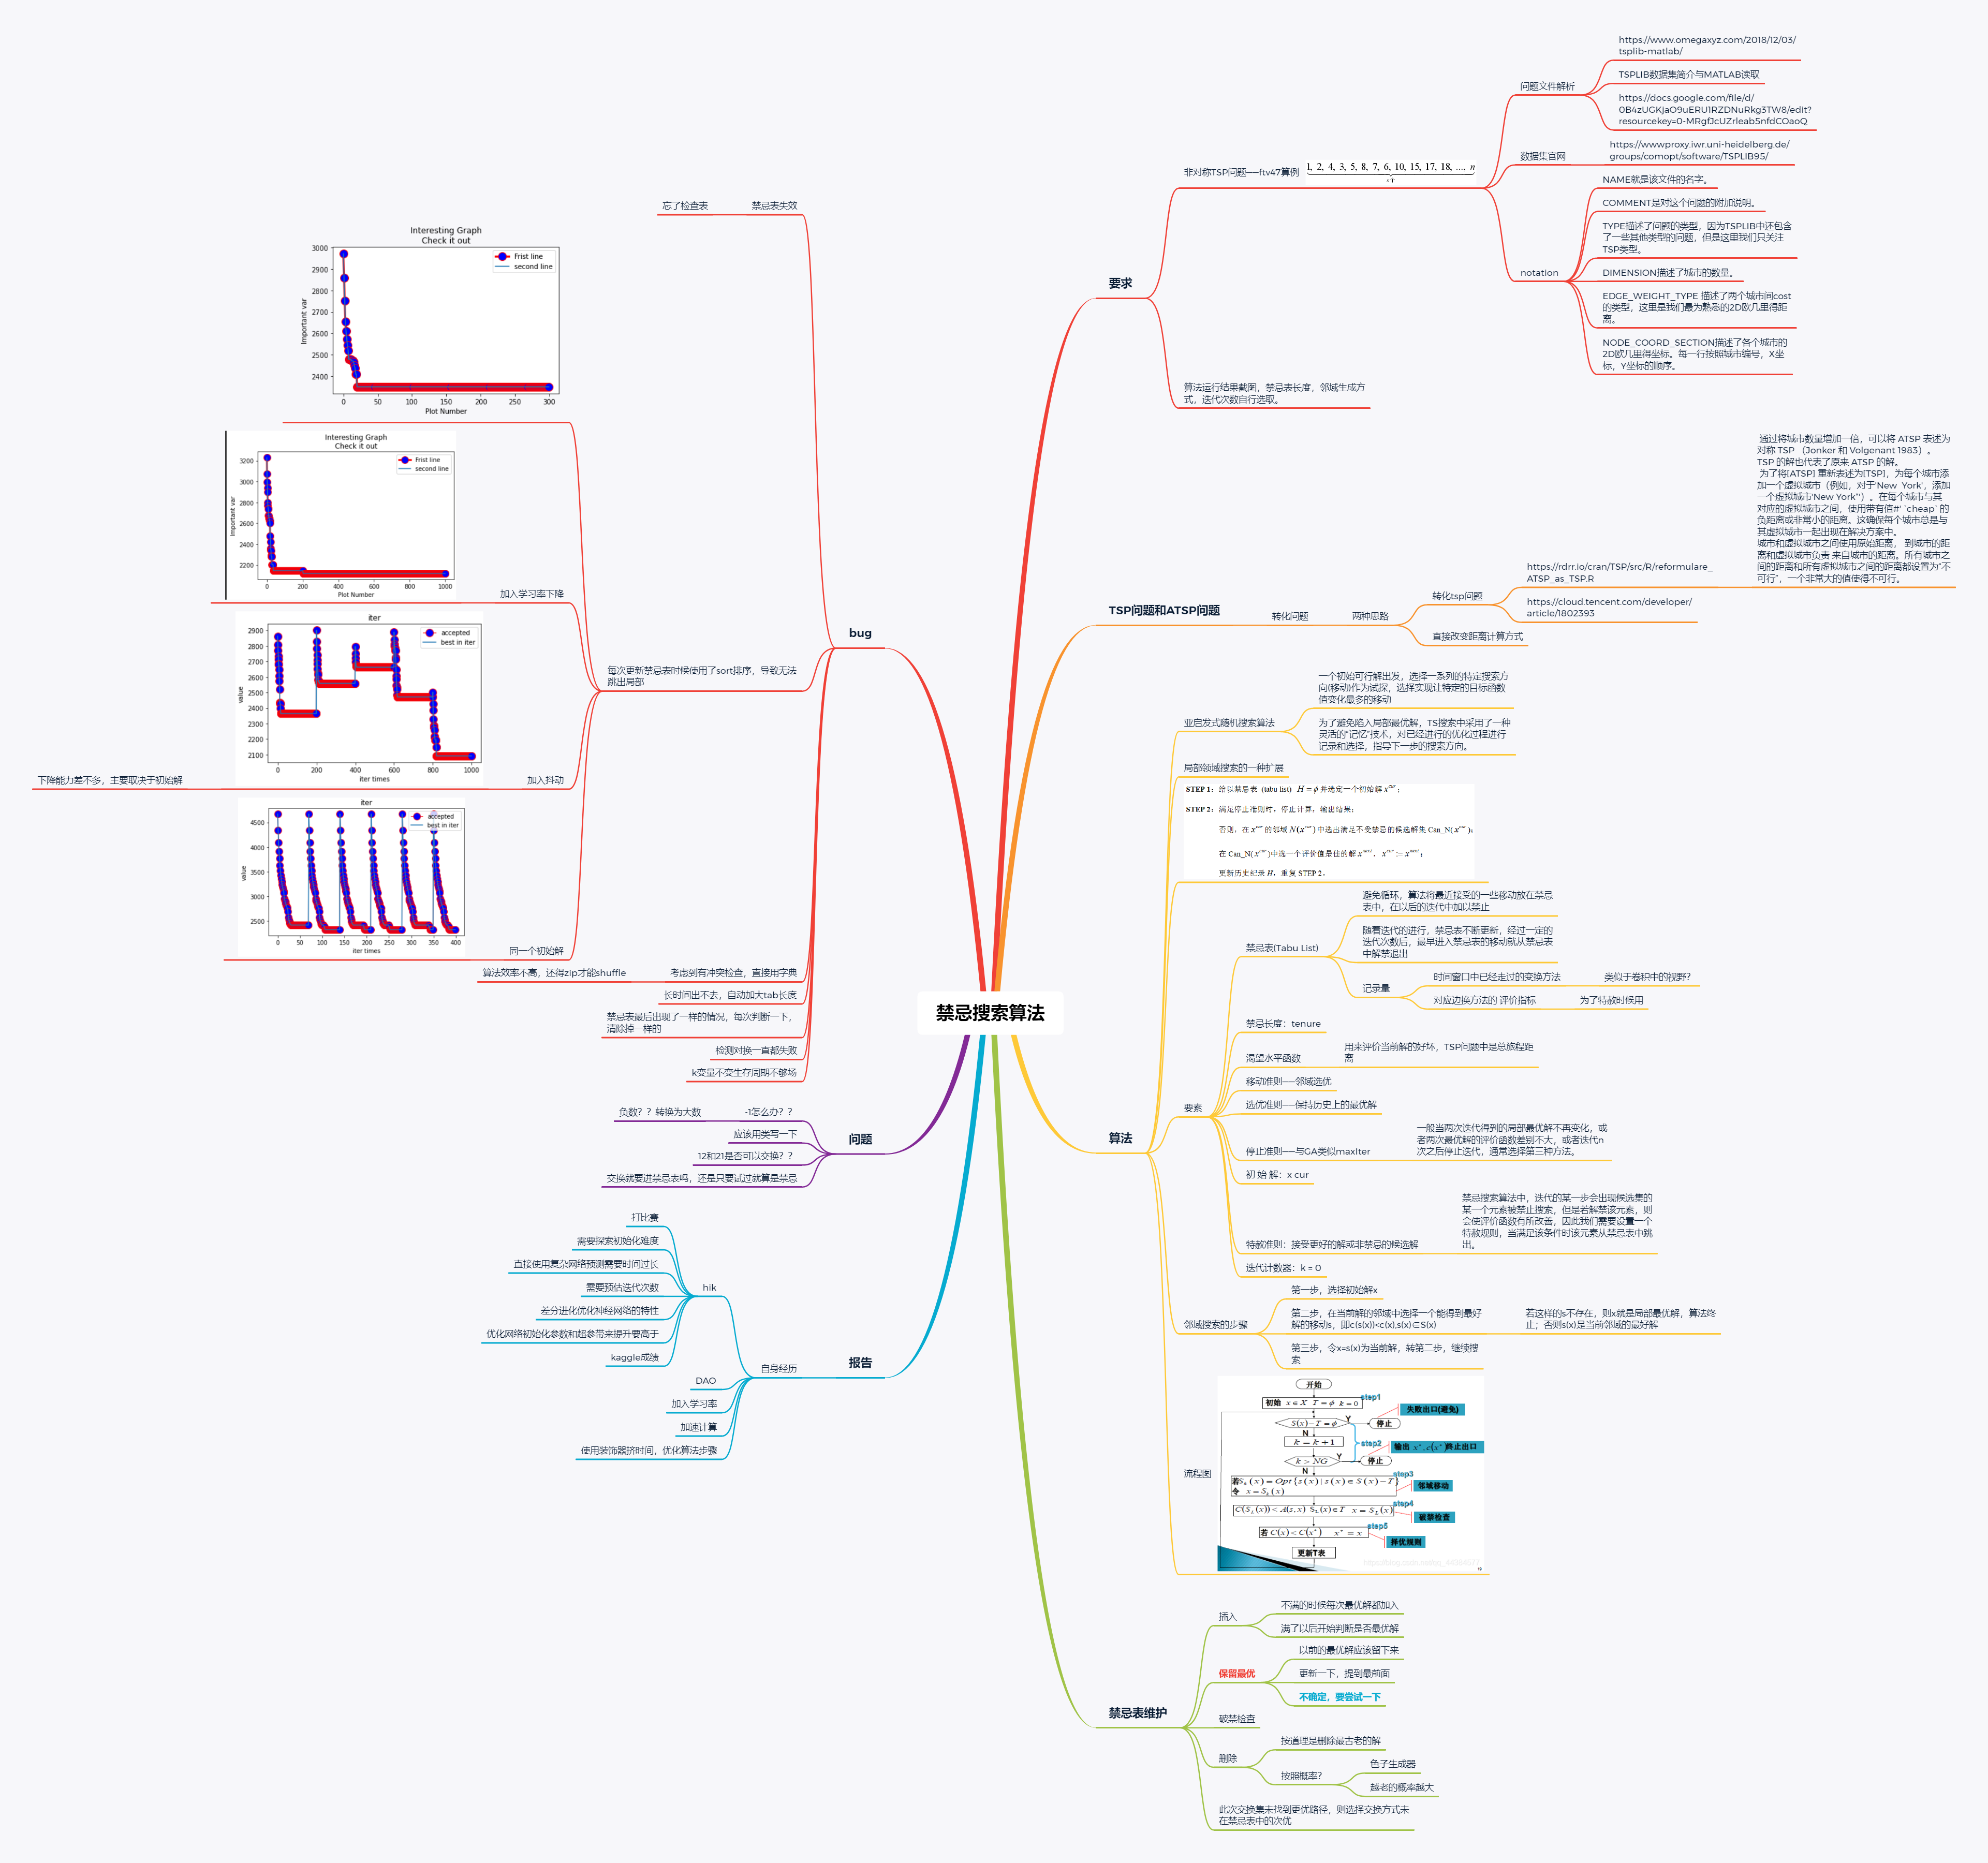
\includegraphics[width=1\textwidth]{figure/禁忌搜索算法.png} %1.png是图片文件的相对路径
  \caption{禁忌搜索算法求解TSP问题思路} %caption是图片的标题
  \label{img:禁忌搜索算法} %此处的label相当于一个图片的专属标志,目的是方便上下文的引用
\end{figure}

\begin{figure}[ht]
  \centering
  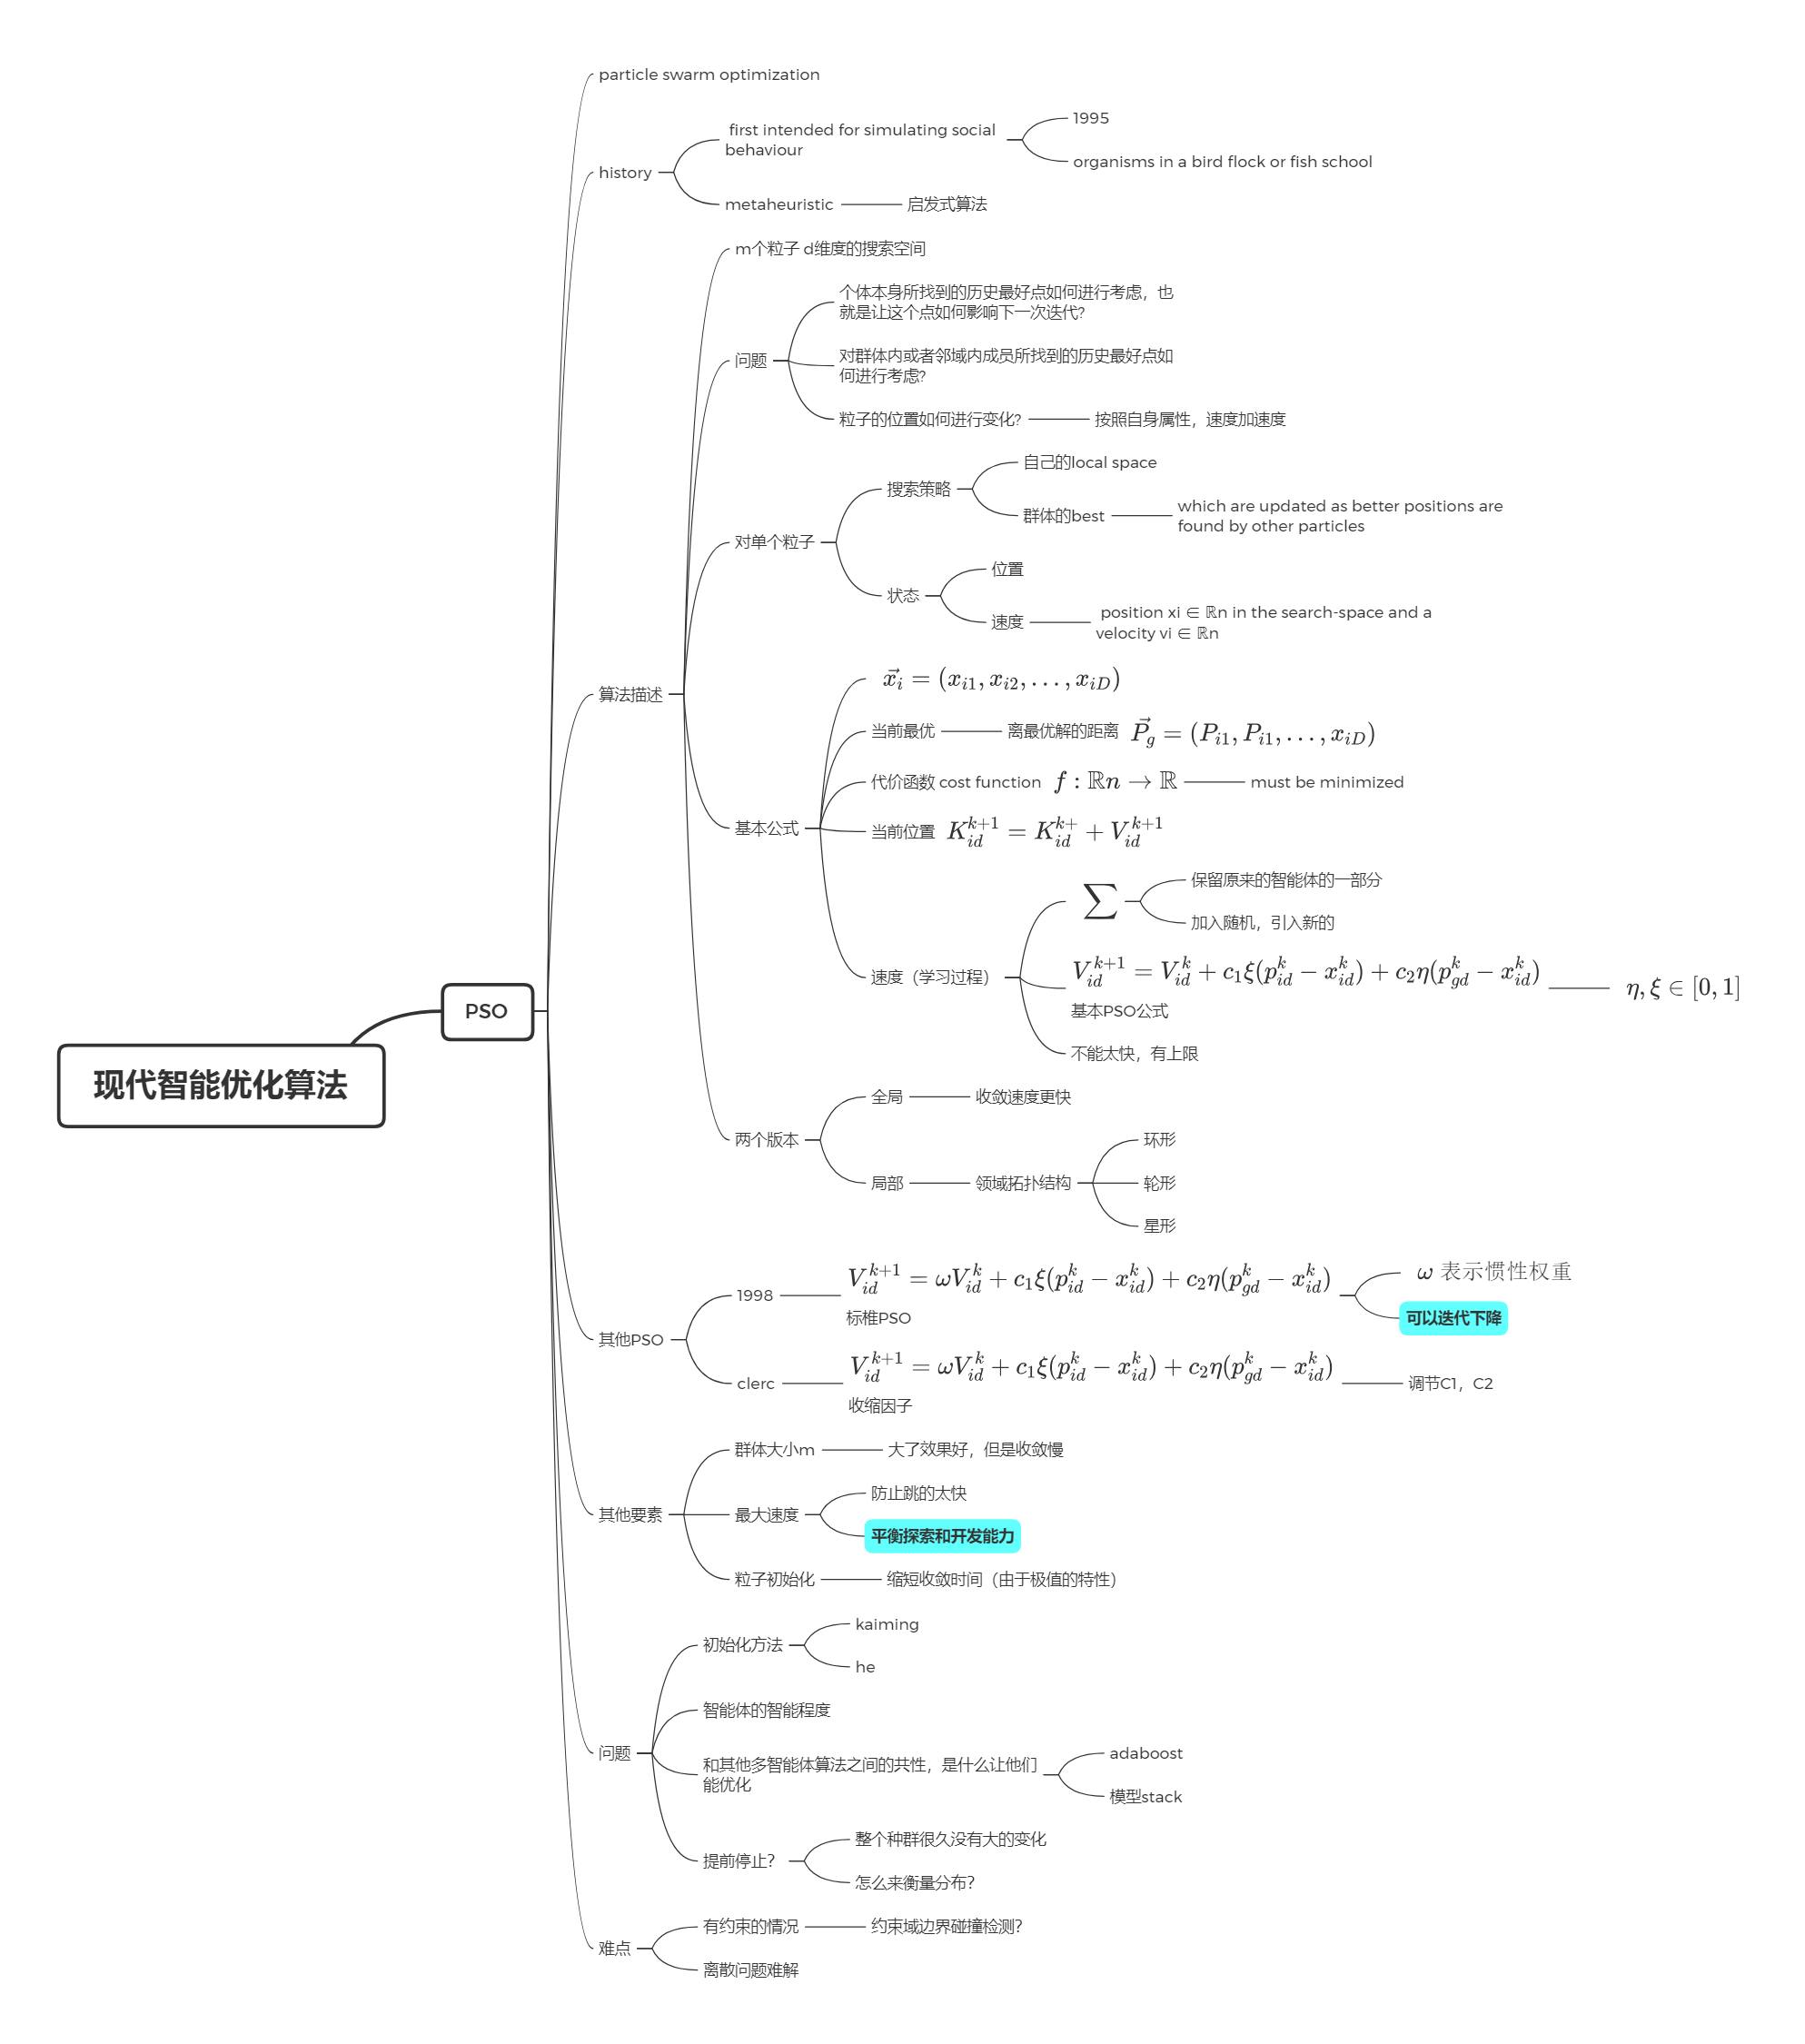
\includegraphics[width=1\textwidth]{figure/PSO/现代智能优化算法——PSO笔记.png} %1.png是图片文件的相对路径
  \caption{PSO求解 TSP 问题思路} %caption是图片的标题
  \label{img:PSO笔记} %此处的label相当于一个图片的专属标志,目的是方便上下文的引用
\end{figure}



\end{document}

